\begin{frame}
	\frametitle{Monop\'olio Natural}
	Vamos imaginar a seguinte situa\c c\~ao:
	\begin{itemize}
		\setlength{\itemsep}{1.5em}
		\item Uma empresa, com custo marginal $c$ produz sozinha, otimamente $N$ unidades de um bem desejado pela sociedade
		\item Admita que a procura por esse bem seja $Q(p)$, e a procura inversa $P(q)$, ambas lineares.
	\end{itemize}
\end{frame}

\begin{frame}
	\frametitle{Monop\'olio Natural}
	\begin{center}
		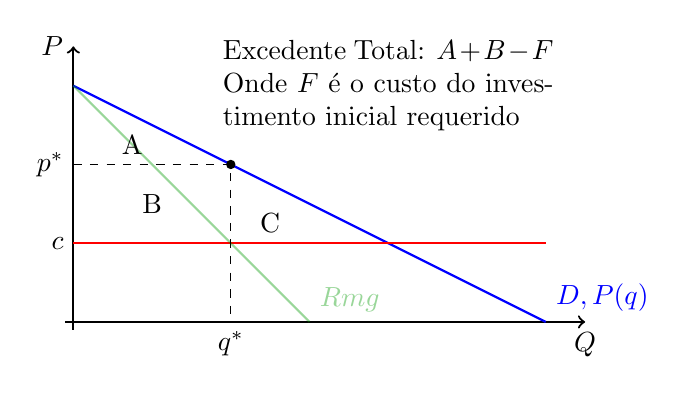
\begin{tikzpicture}[
			declare function = {
				d(\x) = 3-0.5*\x;
				rmg(\x) = 3-\x;
				c(\x) = 1;
			}]

			\def\q{2}

			\draw[->,thick] (-0.1,-0) -- (6.5,-0) node[below]{$Q$};
			\draw[->,thick] (0,-0.1) -- (0,3.5) node[left]{$P$};

			\draw[blue,thick,variable=\x,domain=0:6] plot (\x,{d(\x)}) node[above right]{$D,P(q)$};
			\draw[red,thick,variable=\x,domain=0:6] plot (\x,{c(\x)});
			\draw(0,{c(0)})node[left]{$c$};

			\onslide<2->{
				\draw[green!60!black,thick,variable=\x,domain=0:3,opacity=0.4] plot (\x,{rmg(\x)})node[above right]{$Rmg$};
			}

			\onslide<3->{
				\draw[dashed] (0,{d(\q)})node[left]{$p^*$} -- (\q,{d(\q)})node[circle,fill,inner sep=1.2]{} -- (\q,0)node[below]{$q^*$};
			}

			\onslide<4->{
				\draw(0.75,2.25) node[]{A};
				\draw(1,1.5) node[]{B};
				\draw(2.5,1.25) node[]{C};
			}

			\onslide<5->{
				\draw(4,3) node[]{\parbox{4.2cm}{Excedente Total: $A+B-F$ Onde $F$ \'e o custo do investimento inicial requerido}};
			}

		\end{tikzpicture}
	\end{center}
\end{frame}

\begin{frame}
	\frametitle{Monop\'olio Natural}
	Admita agora que entra uma segunda empresa, e por efeitos da concorr\^encia, o pre\c co desce ao n\'ivel do custo marginal:\[p^*=c\] Teremos ent\~ao a seguinte situa\c c\~ao:
\end{frame}

\begin{frame}
	\frametitle{Monop\'olio Natural}
	\begin{center}
		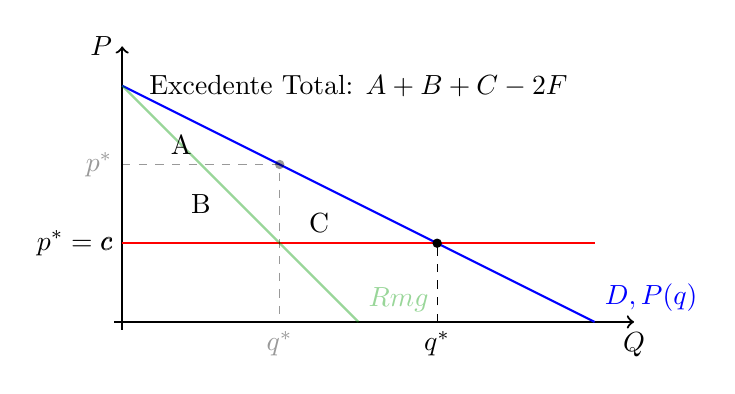
\begin{tikzpicture}[
			declare function = {
				d(\x) = 3-0.5*\x;
				rmg(\x) = 3-\x;
				c(\x) = 1;
			}]

			\def\q{2}
			\def\qe{4}

			\draw[->,thick] (-0.1,-0) -- (6.5,-0) node[below]{$Q$};
			\draw[->,thick] (0,-0.1) -- (0,3.5) node[left]{$P$};

			\draw[blue,thick,variable=\x,domain=0:6] plot (\x,{d(\x)}) node[above right]{$D,P(q)$};
			\draw[red,thick,variable=\x,domain=0:6] plot (\x,{c(\x)});
			\onslide<1>{
				\draw(0,{c(0)})node[left]{$c$};
			}

			\draw[green!60!black,thick,variable=\x,domain=0:3,opacity=0.4] plot (\x,{rmg(\x)})node[above right]{$Rmg$};

			\draw[dashed,opacity=0.4] (0,{d(\q)})node[left]{$p^*$} -- (\q,{d(\q)})node[circle,fill,inner sep=1.2]{} -- (\q,0)node[below]{$q^*$};

			\draw(0.75,2.25) node[]{A};
			\draw(1,1.5) node[]{B};
			\draw(2.5,1.25) node[]{C};

			\onslide<2->{
				\draw[dashed] (\qe,0)node[below]{$q^*$} -- (\qe,{d(\qe)})node[circle,fill,inner sep=1.2]{};
				\draw(0,{c(0)})node[left]{$p^*=c$};
			}

			\onslide<3->{
				\draw(3,3) node[]{Excedente Total: $A+B+C-2F$};
			}

		\end{tikzpicture}
	\end{center}
\end{frame}

\begin{frame}
	\frametitle{Monop\'olio Natural}
	Melhorou a situa\c c\~ao? \onslide<2->{Vejamos:
	\begin{align*}
		A+B+C-2F&>A+B-F\\
		C-F&>0\\
		C&>F
	\end{align*}
	}
	\onslide<3->{
	Ou seja, isto s\'o representa uma melhoria se os custos do investimento inicial necess\'ario foram menores que a \'area $C$, em outras palavras n\~ao \'e sempre o caso que acabar com um monop\'olio seja uma melhoria para o bem estar!
	}
\end{frame}

\begin{frame}
	\frametitle{Monop\'olio Natural}
	Economias de Escala em conjunto com uma procura de mercado pequena, podem reunir condi\c c\~oes para ter um monop\'olio natural, ou seja, apenas uma empresa \'e economicamente vi\'avel, porque consegue ter custos menores ao concentrar a produ\c c\`ao - subaditividade de custos na ind\'ustria.
\end{frame}

\begin{frame}
	\frametitle{Monop\'olio Natural}
	\begin{aquote}{Beaumol, AER 1977}
		A subaditividade da fun\c c\~ao de custos \'e condi\c c\`ao necess\'aria e suficiente para que um sector seja considerado monop\'olio natural.
	\end{aquote}
\end{frame}

\begin{frame}
	\frametitle{Monop\'olio Natural}
	A fun\c c\~ao de custos \'e \textbf{subaditiva} se o custo de produzir a quantidade $q$ com mais do que uma empresa \'e superior ao custo de produzir a mesma quantidade com s\'o uma empresa.
\end{frame}

\begin{frame}
	\frametitle{Monop\'olio Natural}
	Exemplo:
	\begin{itemize}
		\item A extens\~ao de Economias de Escala na produ\c c\~ao de energia el\'etrica \'e a mesma em qualquer parte do mundo, porque isso depende da tecnologia.\pause
		\item Num pa\'is pequeno (ex. Luxemburgo), a produ\c c\~ao de energia el\'etrica pode ser um monop\'olio natural, mas certamente n\~ao o \'e num pa\'is grande, com grande procura (ex. EUA), onde a produ\c c\~ao da quantidade procurada pode n\~ao ter custos m\'edios (na ind\'ustria) minimizados apenas com uma empresa.\pause
	\end{itemize}
	Em ambos os pa\'ises, a extens\~ao de Economias de Escala \'e semelhante, mas num caso haver\'a monop\'olio natural, noutro caso n\~ao (depende da dimens\~ao da Procura)
\end{frame}

\begin{frame}
	\frametitle{Qual o problema dos \emph{\underline{monop\'olios}}?}
	\begin{itemize}
		\item O equil\'ibrio de um mercado concorrencial maximiza o bem-estar conjunto das empresas e dos consumidores (Excedente econ\'omico), isto \'e:\pause
		\begin{itemize}
			\item As empresas escolhem a tecnologia otimamente, dados os pre\c cos dos fatores\pause
			\item Produzem o que os consumidores mais valorizam\pause
			\item Efici\^encia de Custos: output \'e produzido ao custo de oportunidade m\'inimo, o que exige efici\^encia t\'ecnica ao n\'ivel de cada empresa, mas tamb\'em que cada uma minimize os custos de oportunidade dos fatores.
		\end{itemize}
	\end{itemize}
\end{frame}

\begin{frame}
	\frametitle{Qual o problema dos \emph{\underline{monop\'olios}}?}
	Um monopolista, ao exercer o seu \textbf{poder de mercado}, afasta-se da situa\c c\~ao de equil\'ibrio concorrencial, o que gera uma perda de excedente econ\'omico.
\end{frame}

\begin{frame}
	\frametitle{E se houver um monop\'olio natural?}
	\'E prefer\'ivel haver um monop\'olio natural do que n\~ao existir mercado...\par\pause
	\vspace{0.4cm}
	Para evitar que a empresa ``abuse'' do consumidor, normalmente h\'a regula\c c\~ao de pre\c cos(pre\c co m\'aximo, por exemplo), j\'a que a situa\c c\~ao de monop\'olio natural normalmente surge em sectores ligados a infraestruturas que garantem servi\c cos p\'ublicos, onde n\~ao \'e eticamente aceit\'avel praticar-se pre\c cos muito altos.
\end{frame}

\begin{frame}
	\frametitle{Regula\c c\~ao de Pre\c cos}
	Uma solu\c c\~ao frequentemente usada \'e regular para que o monopolista cobre um pre\c co igual ao custo m\'edio de produ\c c\~ao, ficando na pr\' atica com lucro zero.\par
	
	\vspace{0.3cm}

	\'E a situa\c c\~ao de 2\textsuperscript{nd} Best, j\'a que n\~ao \'e vi\'avel ter $P=Cmg$ (1\textsuperscript{st} Best) - Pre\c cos de Ramsey.\par
	
	\vspace{0.3cm}

	O Estado, para conseguir que as empresas sigam esta pol\'itica, tem de pagar indemniza\c c\~oes compensat\'orias que teoricamente se deveriam aproximar do lucro que as empresas teriam se pudessem cobrar o pre\c co maximizador do lucro.
\end{frame}

\begin{frame}
	Problema?\pause\par
	\vspace{0.5cm}

	{\centering \Large As empresas perdem o incentivo a melhorar a produtividade e baixar os custos!
	}
\end{frame}

\begin{frame}
	Outra solu\c c\~ao implementada tem sido fixar pre\c cos m\'aximos e mante-los a\'i por algum per\'iodo de tempo.\pause\par
	\vspace{0.2cm}

	No come\c co, os \textbf{\underline{pre\c cos s\~ao fixados}} com base nos \textbf{\underline{custos de hoje}} da empresa, a modo da mesma ter lucros baixos ou nulos.\par
	\vspace{0.2cm}
	A empresa por outro lado, agora tem incentivos a melhorar a produtividade, pois assim poder\'a ter lucros pelos anos em que o pre\c co esteja fixo!
\end{frame}

\begin{frame}
	Problema?\pause\par

	\vspace{0.5cm}

	{\centering \Large O Governo tem incentivo a atualizar os pre\c cos depois do per\'iodo prometido para incluir as baixas nos custos, e assim a empresa pode fazer um menor esfor\c co em aumentar a produtividade, pois sabe que maiores baixas nos custos ir\~ao causar pre\c cos m\'aximos menores no pr\'oximo per\'iodo!.
	}
\end{frame}